\title{TASBE Color Model Tutorial}
\documentclass[10pt]{article}
\textwidth 6.5in
\textheight 9in
\oddsidemargin -0.2in
\topmargin -0.5in

\usepackage{graphicx,times,amsmath} % Add all your packages here
\usepackage[all]{xy}
\usepackage{multirow}
\usepackage{graphicx}
\usepackage{color}
\usepackage{tabularx}
\usepackage{url}
\usepackage{amsmath}
\usepackage{amssymb}
\usepackage{multirow}
\usepackage[noend,ruled,linesnumbered]{algorithm2e}
\usepackage[numbers, sort]{natbib}
\usepackage{listings}
\usepackage[svgnames]{xcolor}
%\usepackage{newtxtext}
\definecolor{javared}{rgb}{1,0,0} % for strings
\definecolor{javagreen}{rgb}{0.25,0.5,0.35} % comments
\definecolor{javapurple}{rgb}{0.5,0,0.35} % keywords
\definecolor{javadocblue}{rgb}{0.25,0.35,1} % javadoc
\lstdefinestyle{highlight} {
moredelim=[is][\bfseries\textcolor{javadocblue}]{<<>>}{>><<},
moredelim=[is][\itshape]{!!}{??}
}
\lstset{language=Java,
  keywordstyle=\color{javapurple}\bfseries,
  stringstyle=\color{javared},
  commentstyle=\color{javagreen},
  basicstyle=\tt\small,        % the size of the fonts that are used
                               % for the code
  style=highlight,
  breakatwhitespace=false,         % sets if automatic breaks should only happen at whitespace
  breaklines=true,                 % sets automatic line breaking                   % sets the caption-position to bottom
  extendedchars=true,              % lets you use non-ASCII characters; for 8-bits encodings only, does not work with UTF-8
  showspaces=false,                % show spaces everywhere adding particular underscores; it overrides 'showstringspaces'
  showstringspaces=false,          % underline spaces within strings only
  showtabs=false,                  % show tabs within strings adding particular underscores
  tabsize=2,                     % sets default tabsize to 2 spaces
  numbers=left,
  %frameround=ftff,
  frame=shadowbox,
  rulecolor=\color{black},
  rulesepcolor=\color{gray}
  }
\usepackage{hyperref}
\hypersetup{
    colorlinks=true,
    citecolor=teal,
    linkcolor=olive, % Internal links, those generated by cross-referenced elements    
    urlcolor=blue % Links to web sites
}
\begin{document}
  \setlength{\parindent}{1em}
  \setlength{\parskip}{0em}
  \setlength{\parsep}{0em}

 
This tutorial explains building a \textbf{ColorModel} using the \textit{TASBEFlowAnalytics} software package. A \textbf{ColorModel} improves the precision of flow cytometry measurements by translating raw fcs data to a comparable unit data. 

A previous understanding of Flow Cytometry is assumed within this tutorial. However, resources are available for users new to the subject and can be accessed ~\href{https://github.com/mehersam/TASBEFlowAnalytics/tree/gh-pages/docs/FlowCytometryDocumentation}{here}. 

\section*{Creating A Color Model}

  As a starting point for users, a MATLAB script with an example color model is available ~\href{https://github.com/mehersam/TASBEFlowAnalytics/blob/gh-pages/docs/ColorModelTutorial/make\_color\_model.m}{here}. The script is labeled as \textit{make\_color\_model.m}. Users should proceed to download and open this file using MATLAB or Octave. Additionally, example data files are also provided to create the \textbf{ColorModel} and are made available~\href{https://github.com/mehersam/TASBEFlowAnalytics/tree/gh-pages/docs/Example Files/}{here}.  

Within the script, the first step is to set up paths for the location of the various data files. This step is optional, but it is more easier for users since full paths don't need to be used every time when referring to the data files. With that note, we will now explain what file paths are set. The first path should be directed to where the fcs data exists. Currently, the script is coded to include the path to the example files that are provided. The second and third path are set to point towards the \textit{bead} and \textit{blank} file path. 

%Need to explain bead and blank files...what are these exactly
  
\begin{minipage}{0.95\textwidth} 
\begin{lstlisting}
stem0312 = '../example_controls/2012-03-12_';
beadfile = [stem0312 'Beads_P3.fcs'];
blankfile = [stem0312 'blank_P3.fcs'];
\end{lstlisting}
\end{minipage}
 
\section*{Autogating}

Next step is to initialize Autogating. First, the autogating filters need to be initilized as shown in line 1. Some key default filter parameters are already set, but they can be modified as needed by the user. For example, the default number of gaussian components which are searched for are two. The components are set to search for one single-cell component and the second component is typically a non-cell or clump component. Line 2 shows how to change the number of searched components.

Additionally, the default channel names are set as \textit{FSC\-A,SSC\-A,FSC\-H,FSC\-W,SSC\-H,SSC\-W}. These channel names can be modified to add more channel or fewer as needed as shown in line 3. Please see the API to see the complete list of filter parameters available.

Once the parameters are set, we can initialize \textit{Autogating} as shown in line 5. The inputs include the location of the blankfile, the parameters, and output directory where graphical figures will be stored.

\begin{minipage}{0.95\textwidth} 
\begin{lstlisting}
AGP = AutogateParameters();
AGP.k_components = 2; 
AGP.channel_names = {'FSC-A', 'SSC-A'}. 

autogate = autodetect_gating(blankfile,AGP,'plots');
\end{lstlisting}
\end{minipage}

\section*{Creating Channels and ColorPairs}

A useful function of the TASBEFlowAnalytics package is its ability for using multi-color controls to convert other colors in MEFL units. In order to begin this process, channels are created for each color being measured. There are three channels being created, \textit{FITC-A}, \textit{PE-Tx-Red-YG-A}, and \textit{Pacific Blue-A}. As shown in line 4, a channel requires a \textit{name}, \textit{wavelength}, \textit{center filter}, and \textit{width filter}.
Additionally, the directory for where the color file exists must be specified as shown in line 6. Functions exist to add details by which a channel can be identified. For example, \lstinline+setPrintName+ and \lstinline+setLineSpec+ are used to set the name the channel is known by and the color which will appear on graphs when referring to that channel. These are optional functions to use.

\begin{minipage}{0.95\textwidth} 
\begin{lstlisting}
channels = {}; colorfiles = {};

channels{1} = Channel('FITC-A', 488, 515, 20);
colorfiles{1} = [stem0312 'EYFP_P3.fcs'];
channels{1} = setPrintName(channels{1}, 'EYFP'); 
channels{1} = setLineSpec(channels{1}, 'y'); 

channels{2} = Channel('PE-Tx-Red-YG-A', 561, 610, 20);
colorfiles{2} = [stem0312 'mkate_P3.fcs'];
channels{2} = setPrintName(channels{2}, 'mKate');
channels{2} = setLineSpec(channels{2}, 'r');


channels{3} = Channel('Pacific Blue-A', 405, 450, 50);
colorfiles{3} = [stem0312 'ebfp2_P3.fcs'];
channels{3} = setPrintName(channels{3}, 'EBFP2');
channels{3} = setLineSpec(channels{3}, 'b');


\end{lstlisting}
\end{minipage}

The next step is to create the \textit{colorpairfiles} which specify which colors are being converted. Line 3 shows how to create an instance of a color pairing. The first two parameters are the colors which are being converted into one another. We see that \textit{FITC-A} and \textit{PE-Tx-Red-YG-A} are the colors being converted. The third parameter is an alternate color which is used to assist in estimating the conversion which in this case is \textit{Pacific Blue-A}. 

\begin{minipage}{0.95\textwidth} 
\begin{lstlisting}
colorpairfiles = {};

colorpairfiles{1} = {channels{1}, channels{2}, channels{3}, [stem0312 'mkate_EBFP2_EYFP_P3.fcs']};
colorpairfiles{2} = {channels{1}, channels{3}, channels{2}, [stem0312 'mkate_EBFP2_EYFP_P3.fcs']};

\end{lstlisting}
\end{minipage}


\section*{Creating The ColorModel}

All of the inputs necessary to make a color model have been created. The next step is to create the model. As shown in line 1, the parameters needed are the bead file, blank file, the created channels, colorfiles, and colorpairfiles. Additionally, some additional functions have been pre-set for the user. In particular, details for the beads used have been specified through the functions \lstinline+set_bead_model+ and \lstinline+set_bead_batch+. Additionally, line 12 shows the function to limit what bead data values are ignored. Currently, the minimum is set such that any data below 10$^2$ is considered too smeared and is discarded. The peak threshold determines the minimum count per bin for something to be considered part of a peak. This value can be adjusted using \lstinline+set_bead_peak_threshold+ as shown in line 13. 


\begin{minipage}{0.95\textwidth} 
\begin{lstlisting}
CM = ColorModel(beadfile, blankfile, channels, colorfiles, colorpairfiles);
CM=set_bead_plot(CM, 2); 
CM=set_translation_plot(CM, true);
CM=set_noise_plot(CM, true);

CM=set_bead_model(CM,'SpheroTech RCP-30-5A'); 
CM=set_bead_batch(CM,'Lot AA01, AA02, AA03, AA04, AB01, AB02, AC01, GAA01-R'); 

CM=set_FITC_channel_name(CM, 'FITC-A');
CM=set_translation_channel_min(CM,[2,2,2]);

CM=set_bead_min(CM, 2);
CM=set_bead_peak_threshold(CM, 1000);

settings = TASBESettings();
settings = setSetting(settings, 'path', 'plots');

CM = add_filter(CM,autogate);

\end{lstlisting}
\end{minipage}

\begin{minipage} {0.95\textwidth} 
\begin{lstlisting}
% Execute and save the model
CM=resolve(CM, settings);
save('-V7','CM120312.mat','CM');
\end{lstlisting}
\end{minipage}

\section*{Discussion of Graphs}
  
After running the model, a series of graphs will be printed to the \textit{plots} directory which should be in the same location as the script for the model. This section aims to discuss each of the graphical outputs. 

The first output to discuss is the \textit{Autogating} graph. Each of the outputs will correspond to each of the colors measured. The figure belows shows the visualization of the side scatter vs. the forward scatter. As previously discussed, the two main components searched include a main cluster of cells and other non-cells cluster. Component 1 points toward the cell cluster and component 2 corresponds to debris identified as a non-cell component. Users can choose to include more components to be identified. Please see the autogating section above. 

\begin{center}
  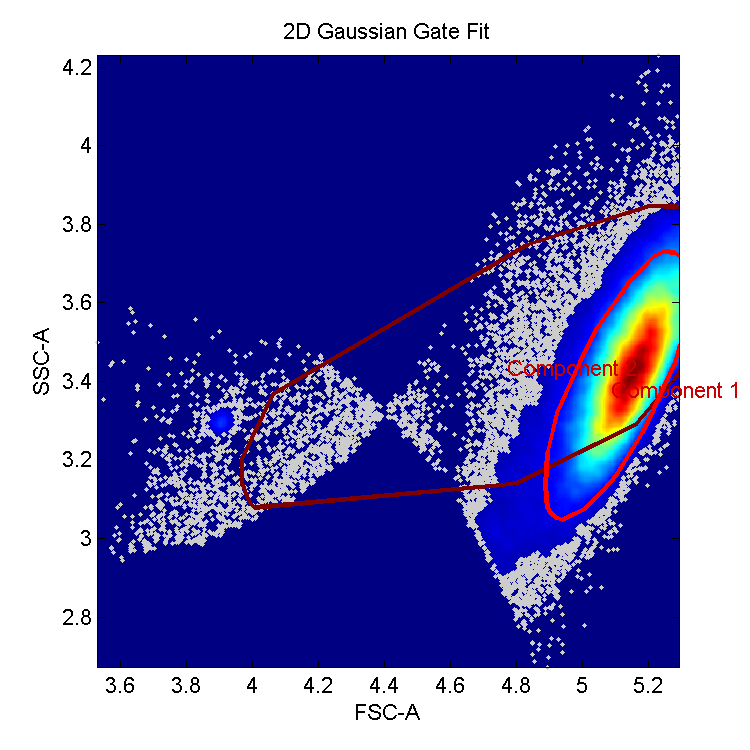
\includegraphics[width=.90\textwidth]{figures/AutomaticGate-FSC-A-vs-SSC-A}
\end{center}

The next figure is the \textit{Autofluoresence} found for the \textit{PE-Tx-Red-YG-A} channel. Users should see a bell-curve with values just below zero and some above. Some possible warnings that might arise from this graph to note. If a majority of the curve exists below zero, then this could be a high autofluorescence within the cells being measured. Alternatively,  a widespread curve could point towards to instrument error. 

\begin{center}
  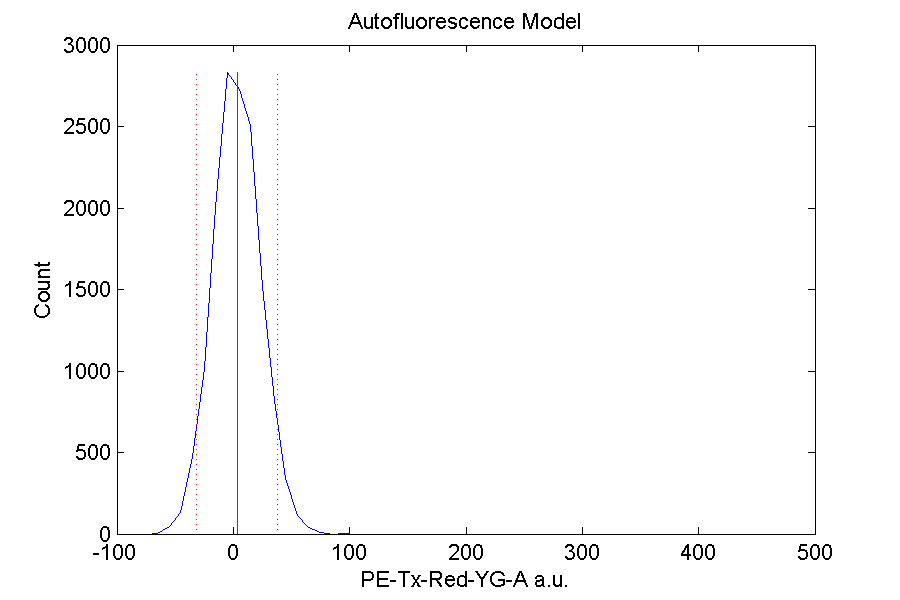
\includegraphics[width=.80\textwidth]{figures/autofluorescence-mKate}
\end{center}

There was one peak selected; however, this graph seems as if part of the peak was excluded. If users would like to extend the range of bead points graphed, then they are able to set the minimum and maximum bead peak range using \lstinline+set\_minimum\_peak+ and \lstinline+set\_maximum\_peak+ functions respectively. This was not actually the case for this graph and extending the minimum will show noisy data that was correctly excluded.   

\begin{center}
  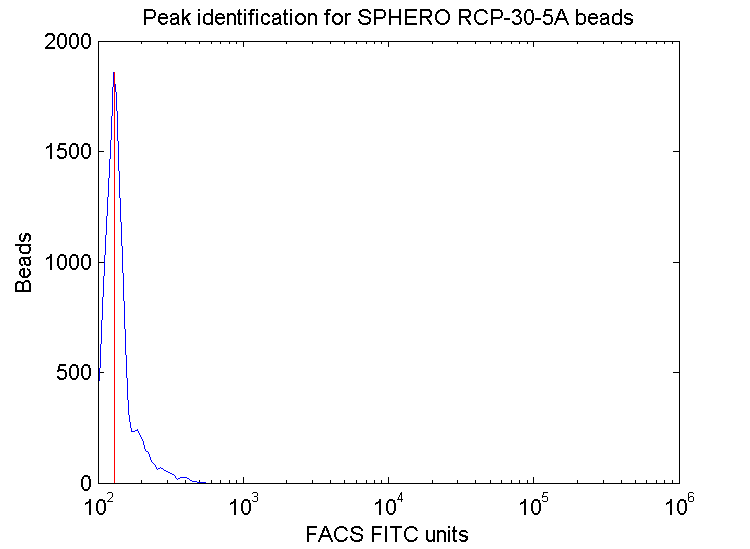
\includegraphics[width=.90\textwidth]{figures/bead-calibration}
\end{center}

There was one peak that was estimated and this can be corroborated with the previous graph. One thing to note is if the \textit{observed} points do not match the \textit{constrained fit} then this could point to the correct peaks not being chosen. 

\begin{center}
  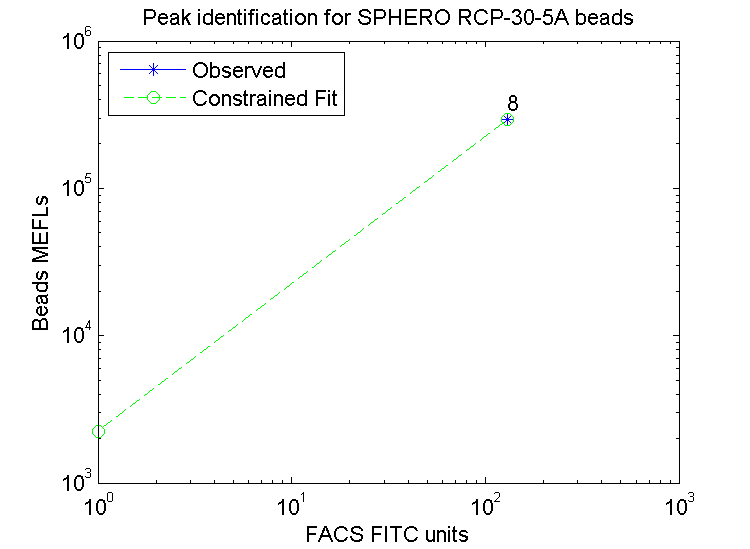
\includegraphics[width=.90\textwidth]{figures/bead-fit-curve}
\end{center}

The last figures show the \textbf{compensation} and \textbf{translation}. The \textbf{compensation} model denotes the rate separation of one color from another. In this case, this model shows the separation of \textit{EYFP} from \textit{mKate}.  
%Talk about error being less than 10

\begin{center}
  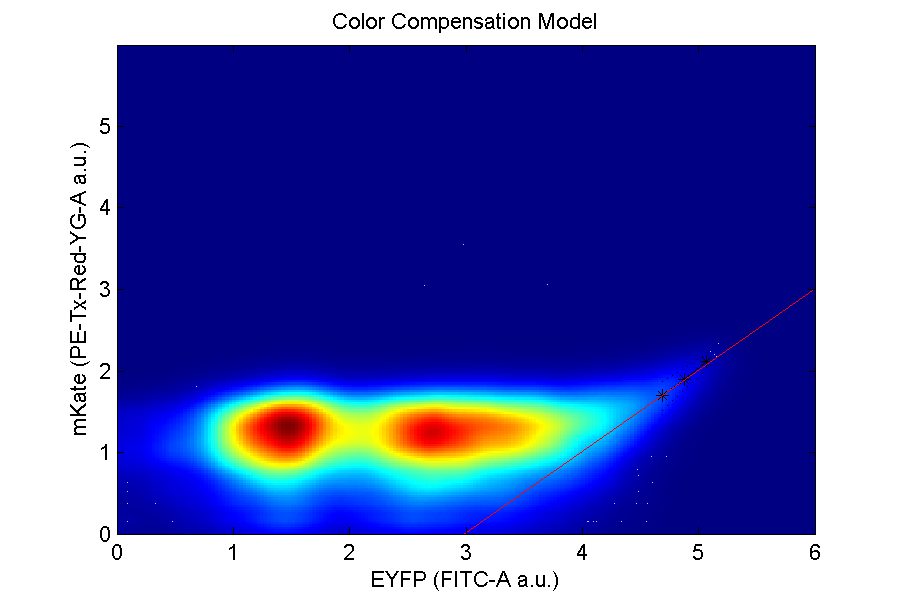
\includegraphics[width=.90\textwidth]{figures/color-compensation-mKate-for-EYFP}
\end{center}


\begin{center}
  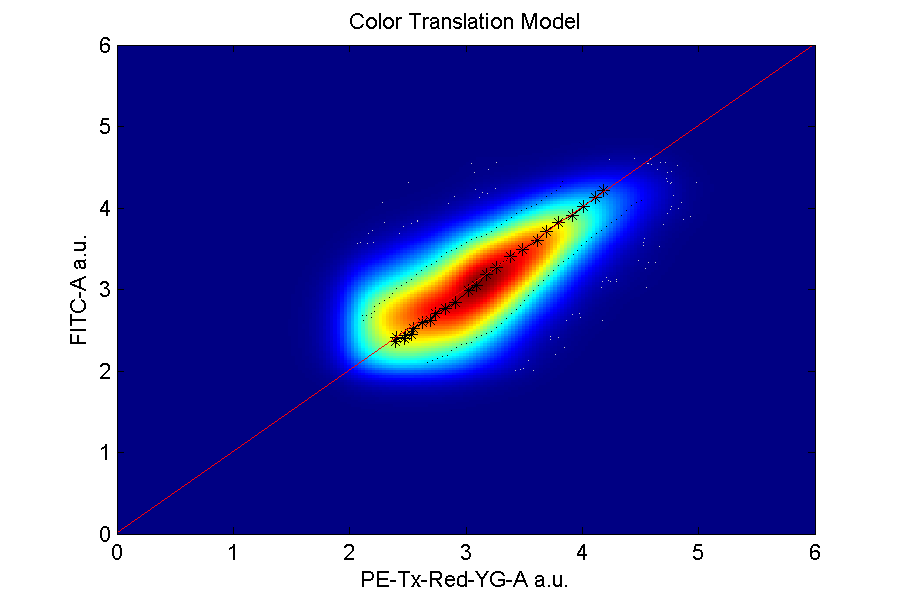
\includegraphics[width=.90\textwidth]{figures/color-translation-mKate-to-EYFP}
\end{center}

  

\end{document}